\part{Assignments}\label{assignments}

\chapter{Project 0}\label{assignment-0}

Project 0 will require you to identify the different software
tools/technologies included in the given attachment and then group them
into the correct layer of categories as indicated on the left-hand side
of the slide.

This homework is worth 5 points.

\slides{Assignments}{Project 0}{5 points}{https://drive.google.com/open?id=0B88HKpainTSfQ2FrUzdKRkM5X0U}

\chapter{Project 1}\label{project-1}

You will need to complete the source code and write a report. Zip your
work into a file with the name username\_project1.zip (replace
`username' with your Group Contact member's username) and submit the
following:

\begin{itemize}
\item
  Complete source code
\item
  \begin{description}
  \item[A document with the following details:]
  \begin{itemize}
  \tightlist
  \item
    Transformation of data during the computations, i.e. data type of
    key, value
  \item
    The data structure used to transfer between Map and Reduce phases
  \item
    How the data flow happens through disk and memory during the
    computation
  \end{itemize}
  \end{description}
\end{itemize}

Only one submission per group is required for Project 1. 
\iffalse
It is due time at 11:59 pm on Feburary 5.
\fi

\setboolean{@twoside}{false}
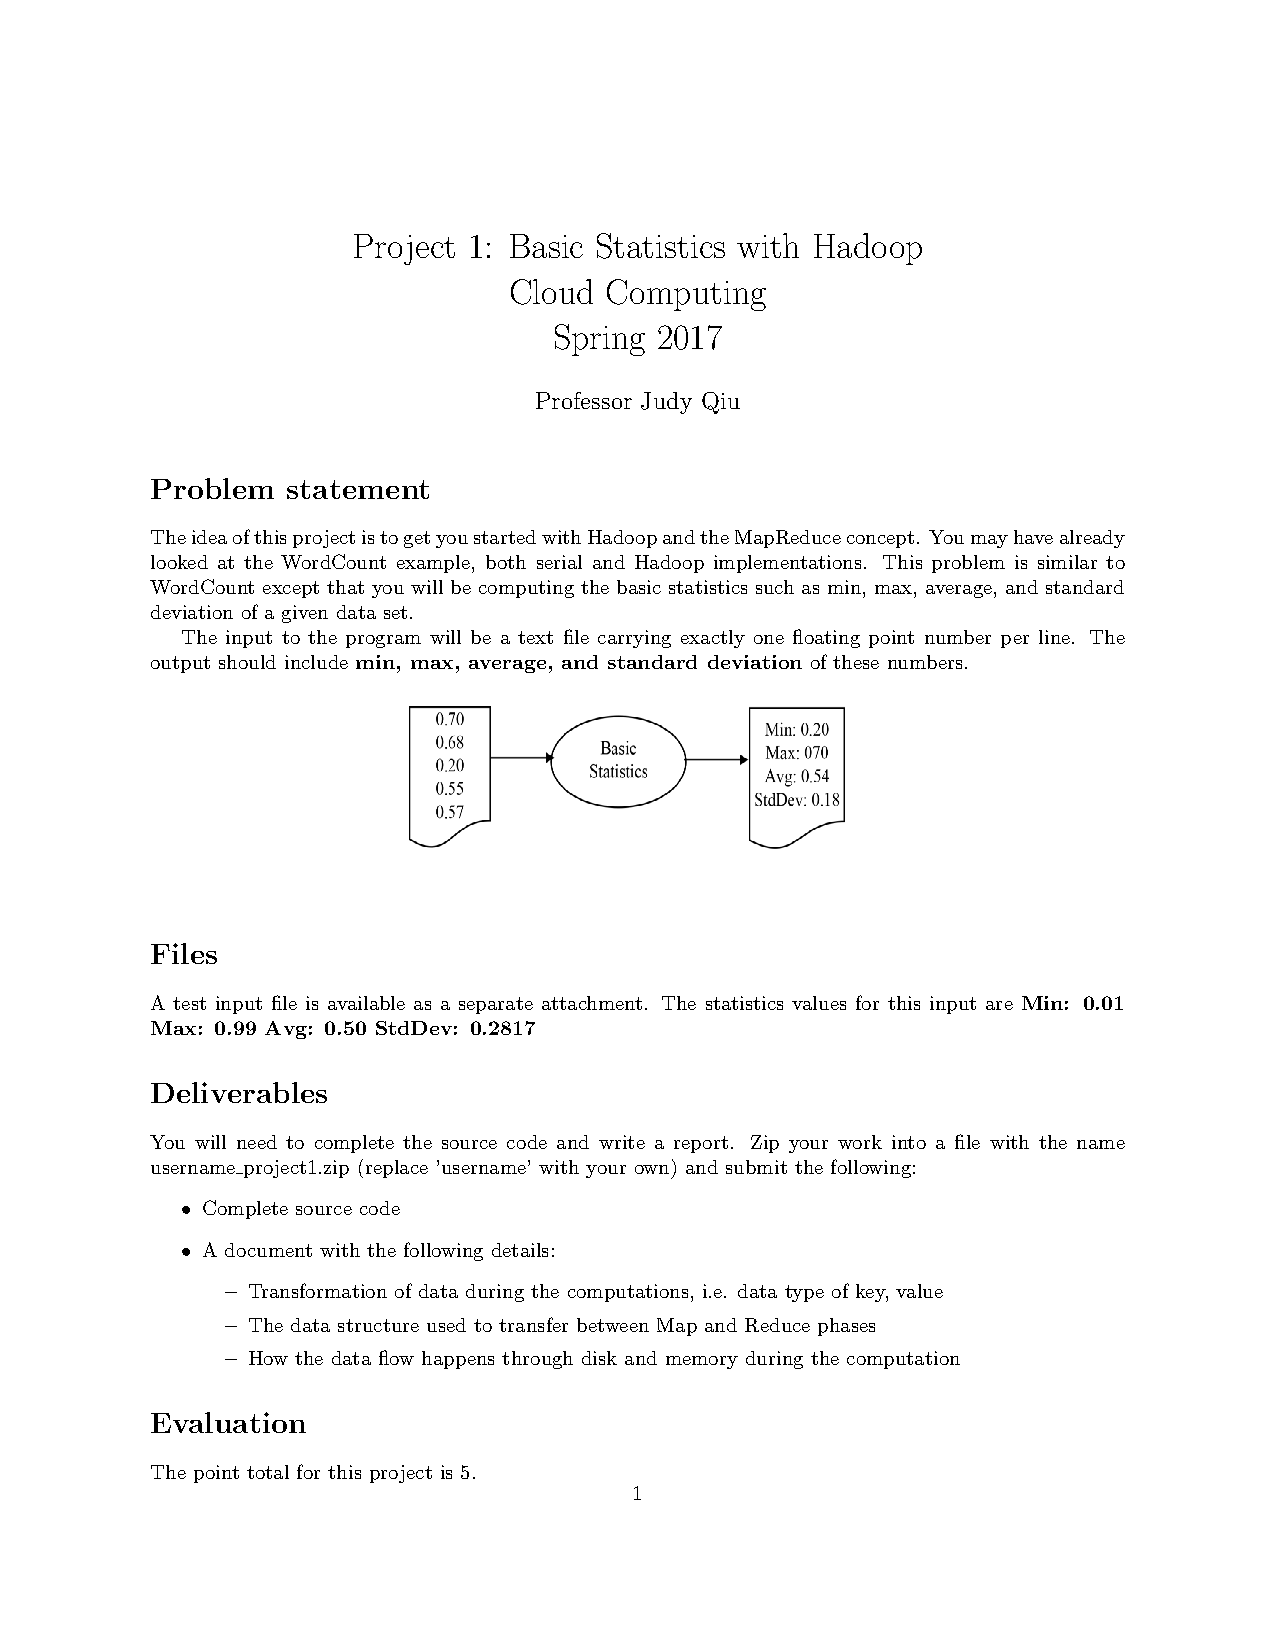
\includepdf[pages=-,pagecommand={},width=\textwidth]{section/icloud/assignment/files/project1.pdf}

\slides{Assignments}{Project 0}{Input Data}{https://drive.google.com/open?id=0B88HKpainTSfcUlZX3BpV05TRDg}

\chapter{Project 2}\label{project-2}

You are required to turn in the following items in a zip file
(username\_HadoopPageRank.zip) in this assignment:

\begin{itemize}
\item
  The source code of Hadoop PageRank you implemented.
\item
  \begin{description}
  \item[Technical report (username\_HadoopPageRank\_report.docx) that
  contains:]
  \begin{itemize}
  \tightlist
  \item
    The description of the main steps and data flow in your program.
  \item
    The output file (username\_HadoopPageRank\_output.txt) which
    contains the first 10 urls along with their ranks.
  \end{itemize}
  \end{description}
\end{itemize}

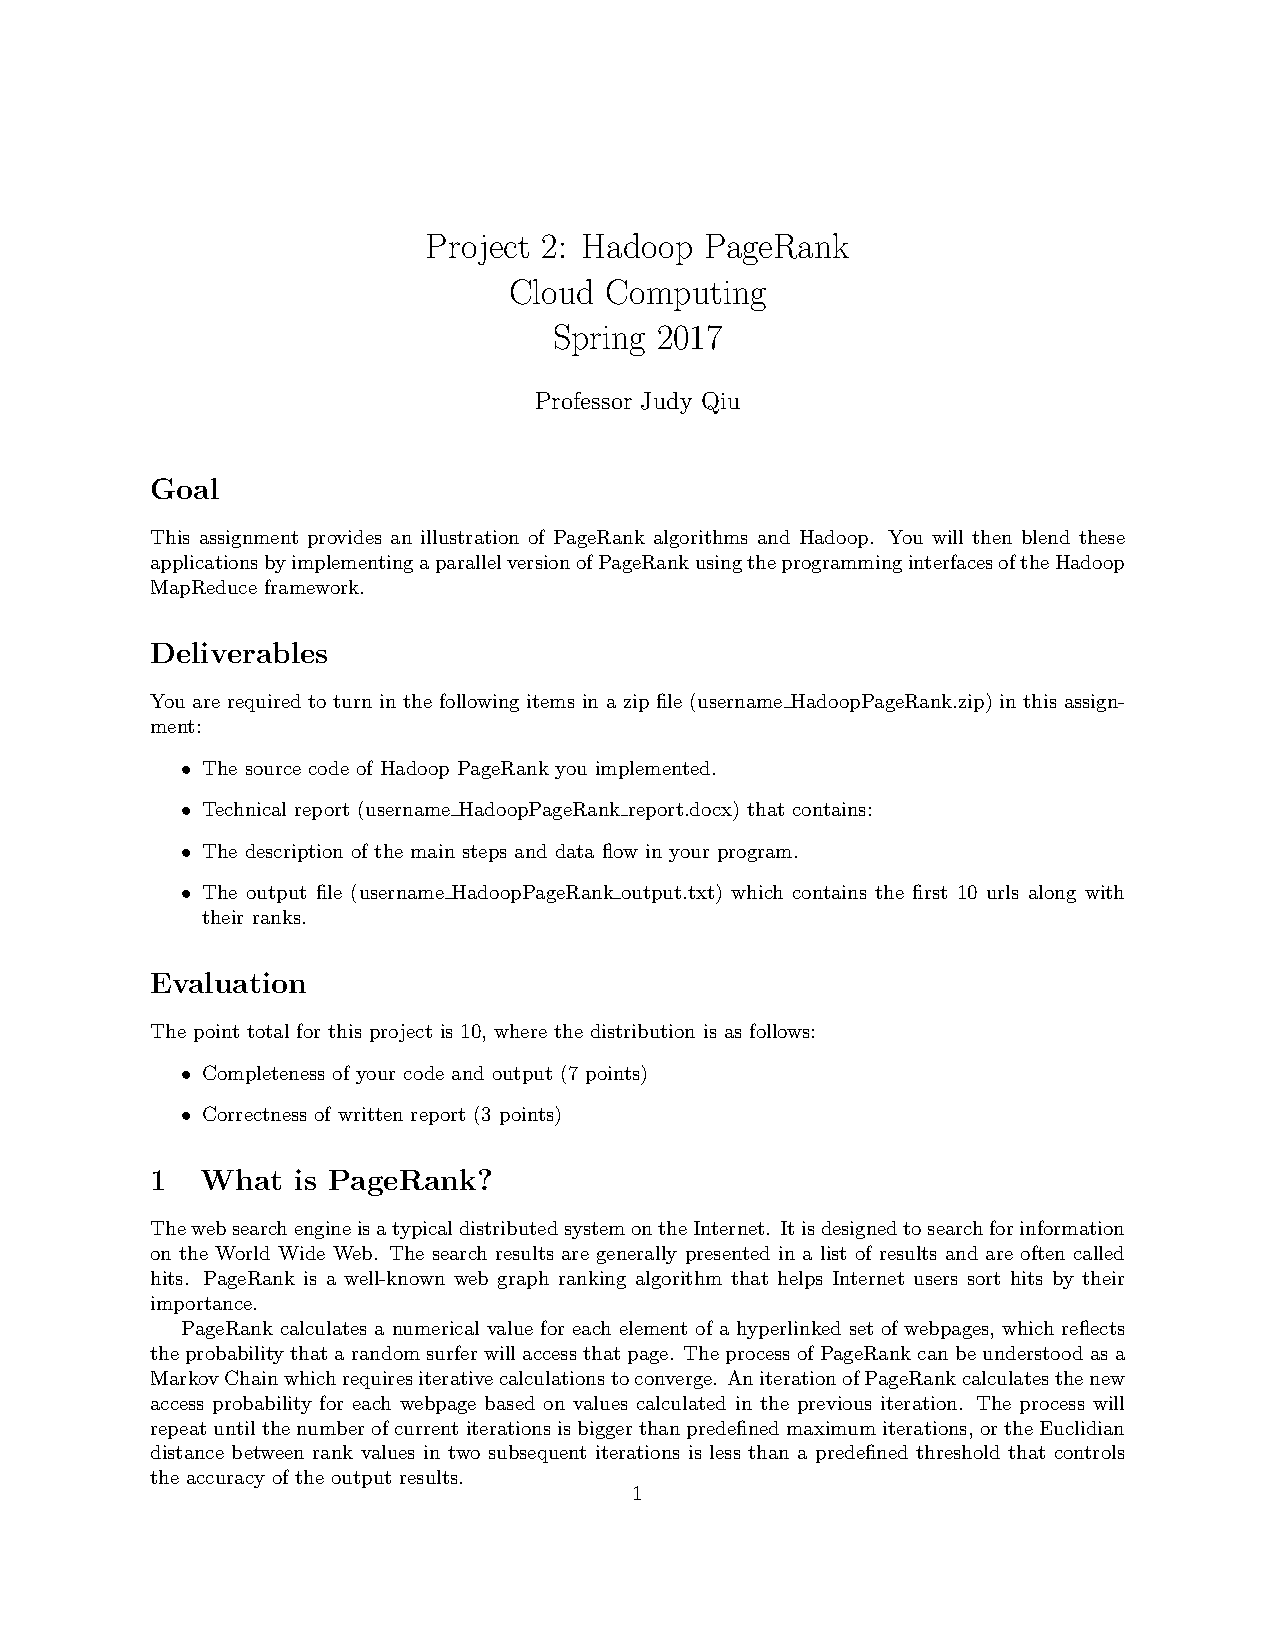
\includepdf[pages=-,pagecommand={},width=\textwidth]{section/icloud/assignment/files/project2.pdf}

\chapter{Project 3}\label{project-3}

Project 3 asks you to implement a bioinformatics application using
Hadoop (Map only) MapReduce framework and write a report about the data
flow and your observations of the program.

You are required to turn in the following items in a zip file
(username\_HadoopBlast.zip) in this assignment:

\begin{itemize}
\tightlist
\item
  The source code of Hadoop Blast you implemented.
\item
  Technical report (username \_HadoopBlast\_report.docx) that answers
  the following questions. - What is Hadoop Distributed Cache and how is
  it used in this program? - Write the two lines that put and get values
  from Distributed cache. Also include the method and class information.
  - In previous projects we used Hadoop's TextInputFormat to feed in the
  file splits line by line to map tasks. In this program, however, we
  want to feed in a whole file to a single map task. What is the
  technique used to achieve this? Also, briefly explain what are the key
  and value pairs you receive as input to a map task and what methods
  are responsible for producing these pairs? - Do you think this
  particular implementation will work if the input files are larger than
  the default HDFS block size? Briefly explain why. [Hint: you can
  test what will happen by concatenating the same input file multiple
  times to create a larger input file in the resources/blast\_input
  folder] - If you wanted to extend this program such that all output
  files will be concatenated into a single file, what key and value
  pairs would you need to emit from the map task? Also, how would you
  use these in the reduce that you would need to add?
\item
  The 4 output FASTA files -- celllines\_1.fa to celllines\_4.fa.
\end{itemize}

Points will be reduced (maximum 0.5 points) if the filename or directory
structure are different from instructed above.

The point total for this project is 3, where the distribution is as
follows:

\begin{itemize}
\tightlist
\item
  Completeness of your code and output (1 points)
\item
  Correctness of written report (2 points)
\end{itemize}

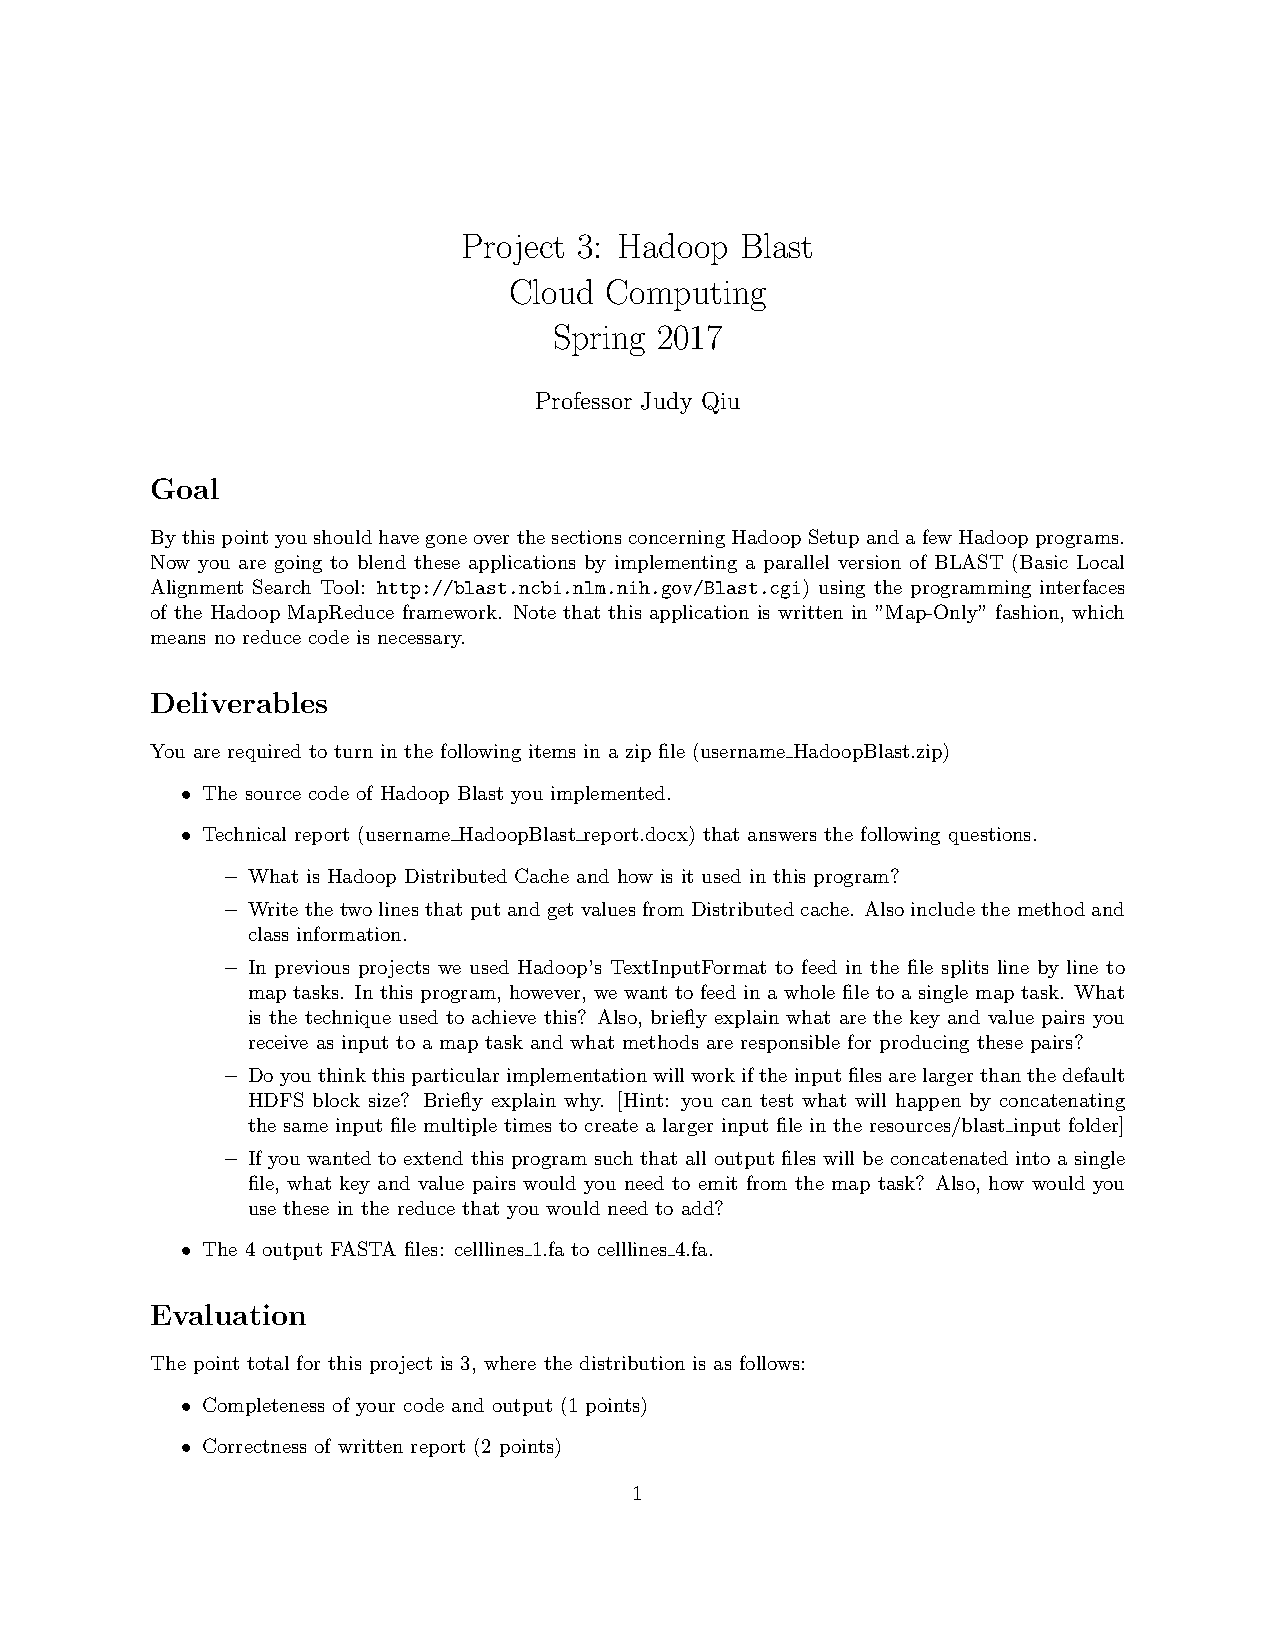
\includepdf[pages=-,pagecommand={},width=\textwidth]{section/icloud/assignment/files/project3.pdf}

\chapter{Project 4}\label{project-4}

Zip your source code and report in a file named username\_project4.zip

The point total for this project is 1.5, where the distribution is as
follows:

\begin{itemize}
\tightlist
\item
  Correctness of your code and output (1 points)
\item
  Completeness of written report (0.5 points)
\end{itemize}

Before you start this project, you need to complete the
Project4 Prerequisite\textless{}files/project4\_pre.pdf\textgreater{}
first. The submission folder for it will be published before the lab
session.

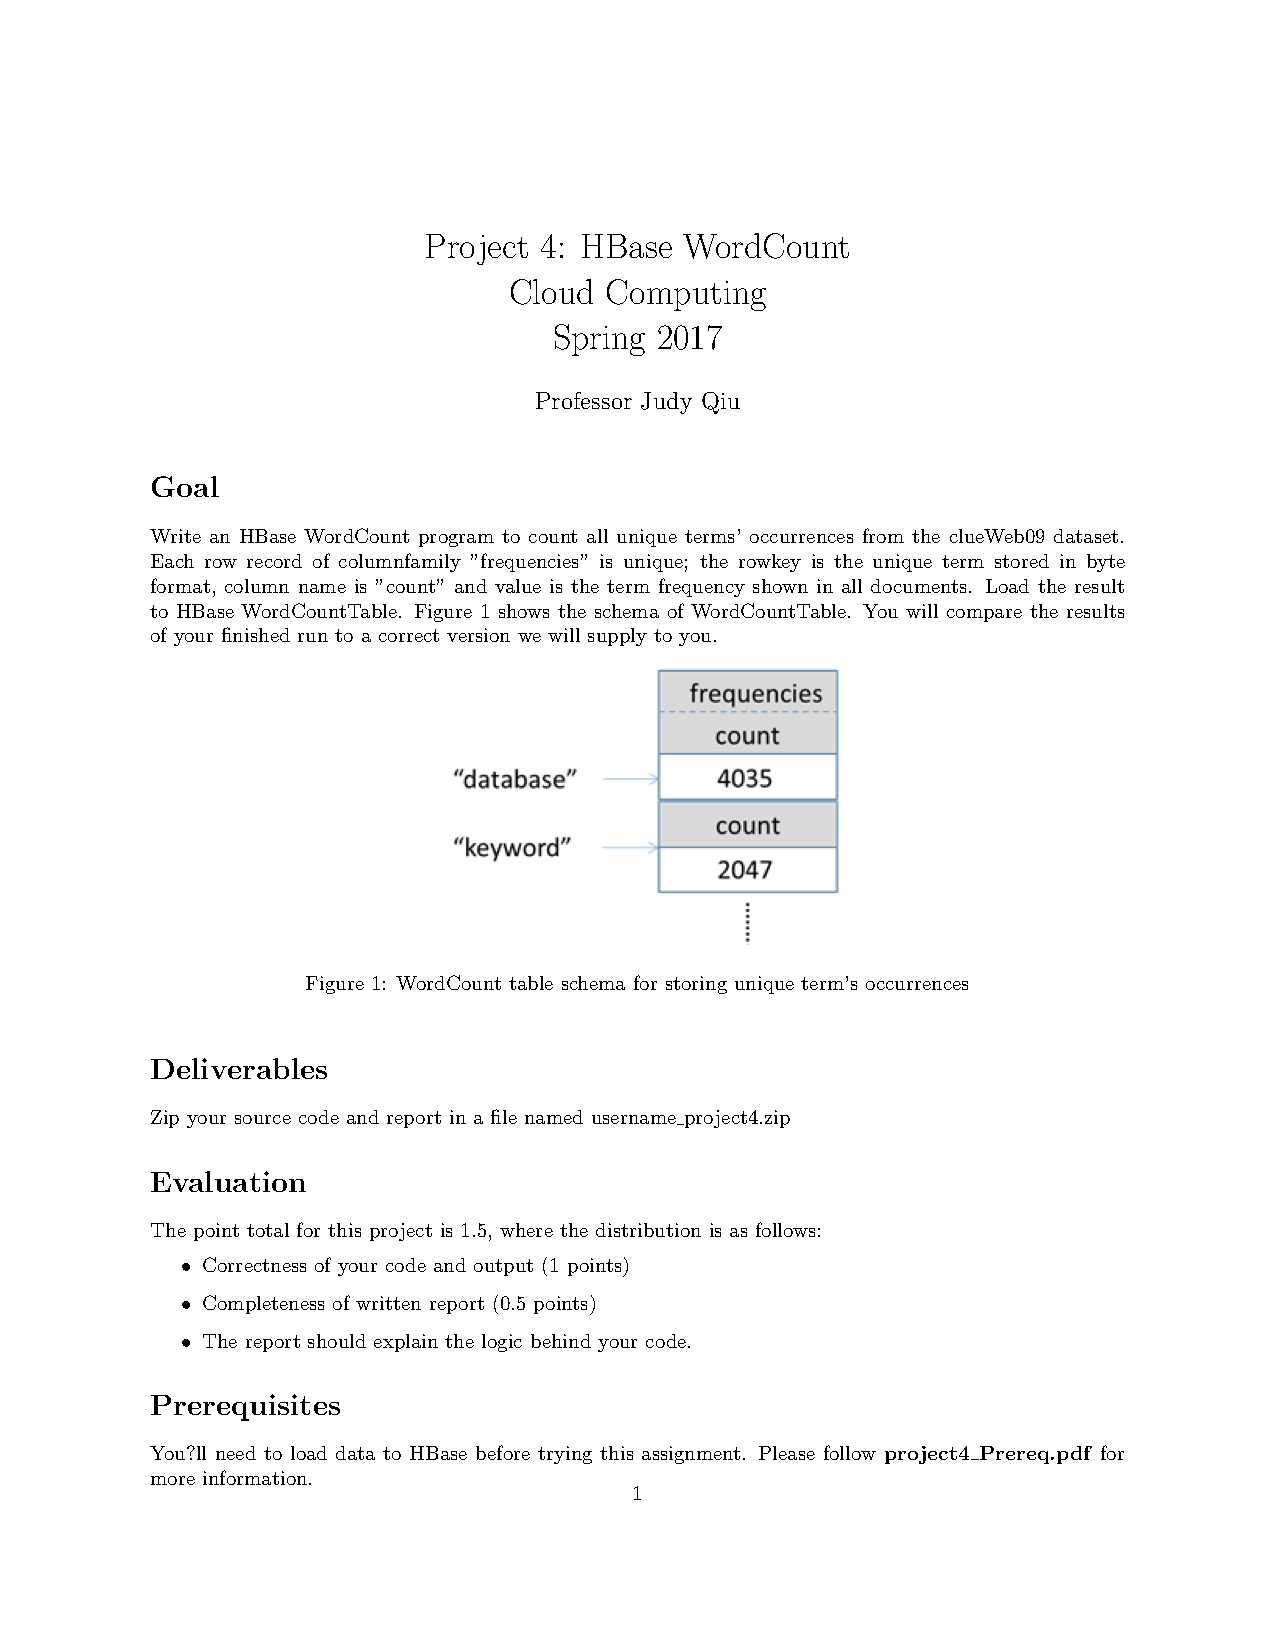
\includepdf[pages=-,pagecommand={},width=\textwidth]{section/icloud/assignment/files/project4.pdf}
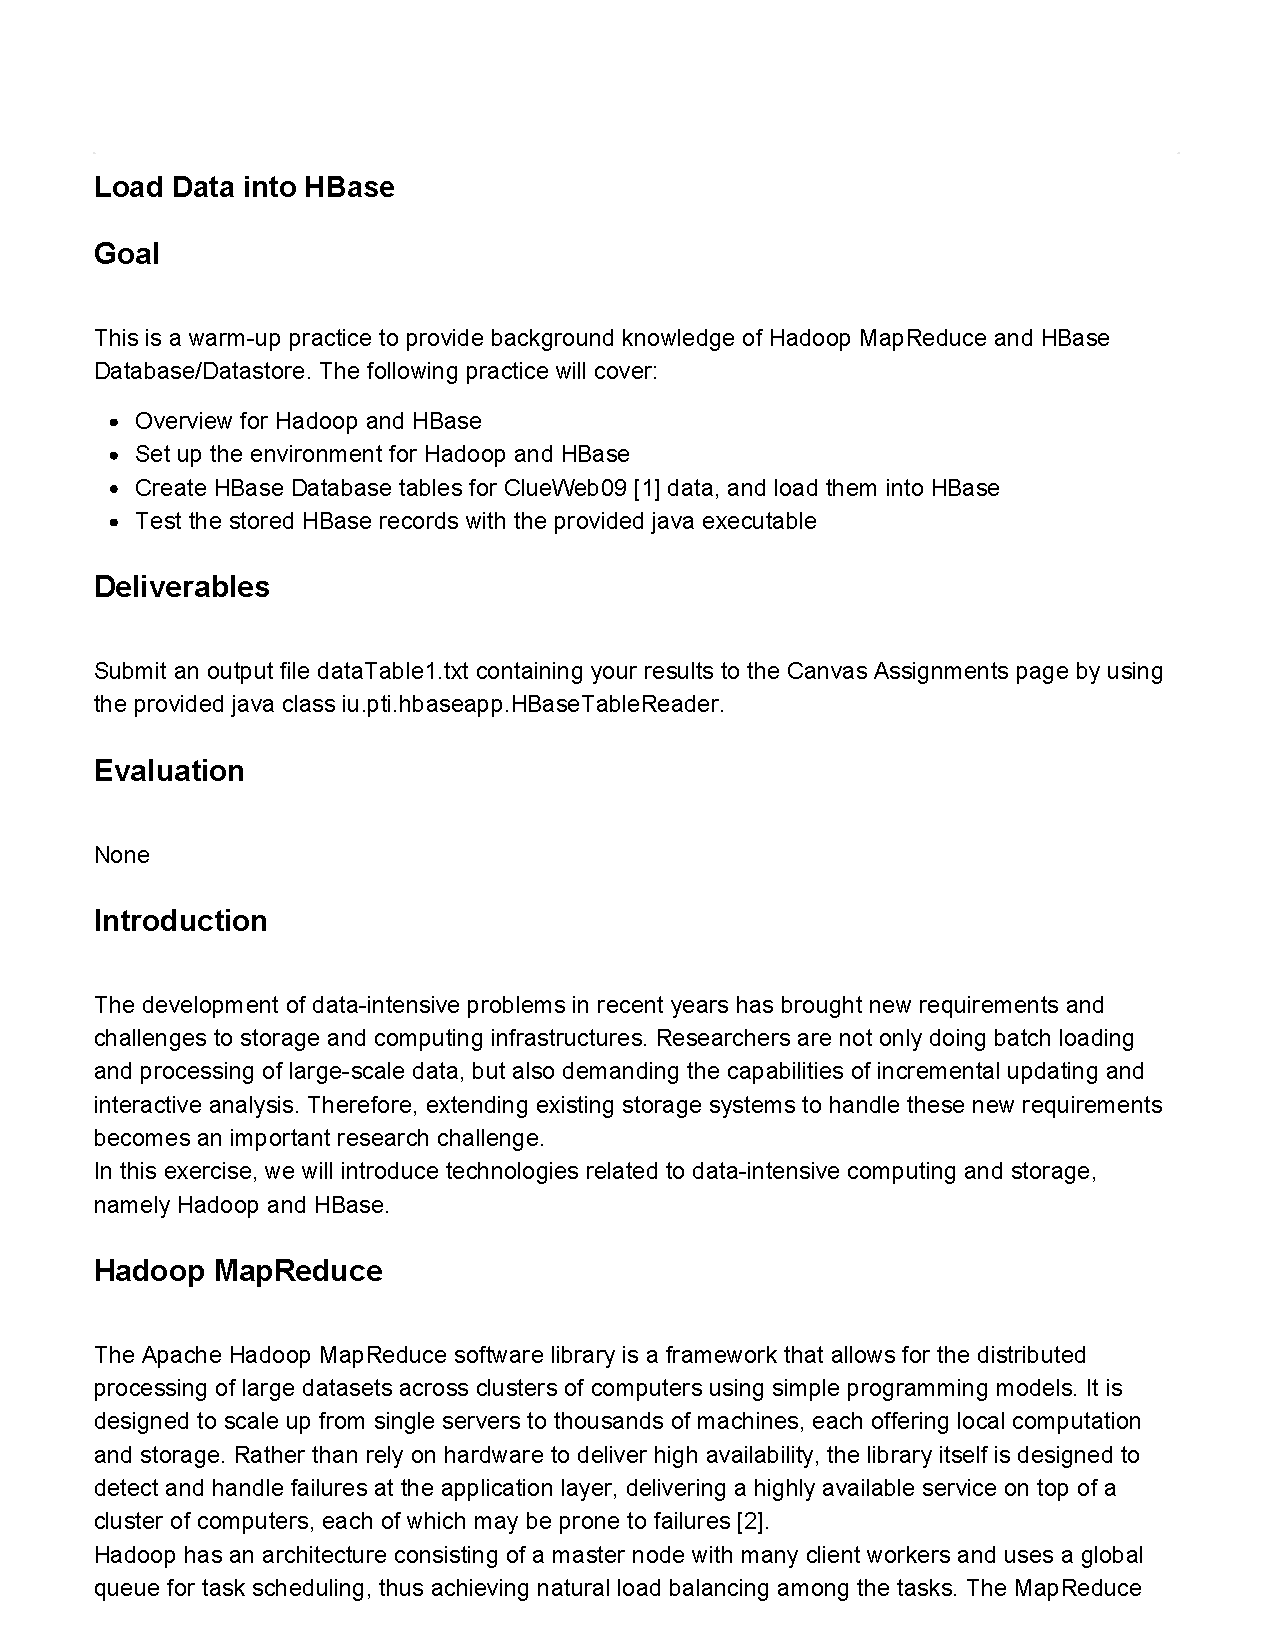
\includepdf[pages=-,pagecommand={},width=\textwidth]{section/icloud/assignment/files/project4_pre.pdf}

\chapter{Project 5}\label{project-5}

Write an HBase FreqIndexBuilder program to build an inverted index table
which has the unique term's occurrences in all documents from the
clueWeb09 dataset. Zip your source code, results and report in a file
named username\_project5.zip. Submit this file to the Canvas submission
page.

\begin{itemize}
\tightlist
\item
  Complete source code
\item
  A written report describing the main steps
\end{itemize}

The point total for this project is 3, where the distribution is as
follows:

\begin{itemize}
\tightlist
\item
  Completeness of your code and output (2 points)
\item
  Correctness of written report (1 points)
\end{itemize}

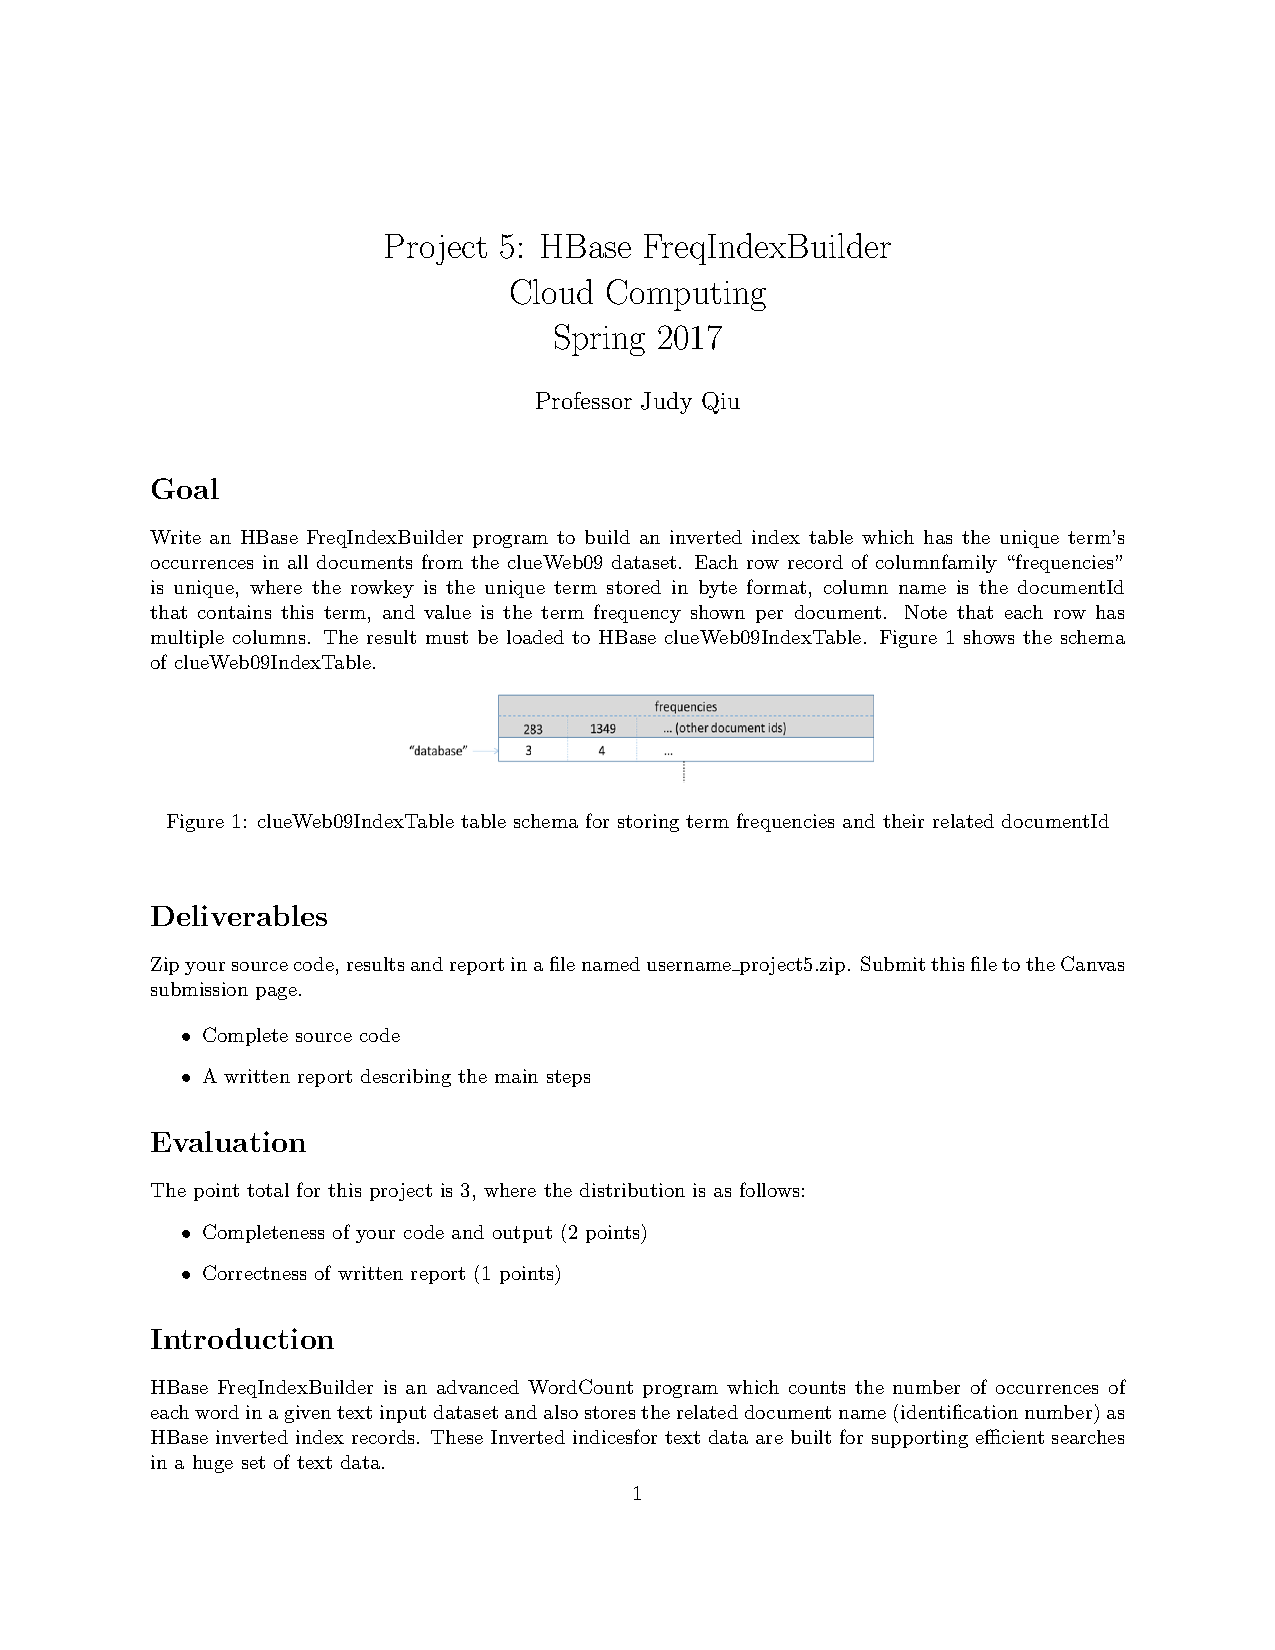
\includepdf[pages=-,pagecommand={},width=\textwidth]{section/icloud/assignment/files/project5.pdf}

\chapter{Project 6}\label{project-6}

After having familiarized yourself with the ``HBase Building an Inverted
Index'' homework and ``PageRank algorithms'' homework, you are ready to
use these applications to test the search engine function from the
packaged executable.

\section{Deliverables}\label{deliverables}

Zip your source code, library, and results in a file named
\href{mailto:username@test-search-engine.zip}{\nolinkurl{username@test-search-engine.zip}}.
Please submit this file to the Canvas Assignments page.

\section{Evaluation}\label{evaluation}

The point total for this project is 6, where the distribution is as
follows:

\begin{itemize}
\tightlist
\item
  Completeness of your code (5 points)
\item
  Correct output (1 points)
\end{itemize}

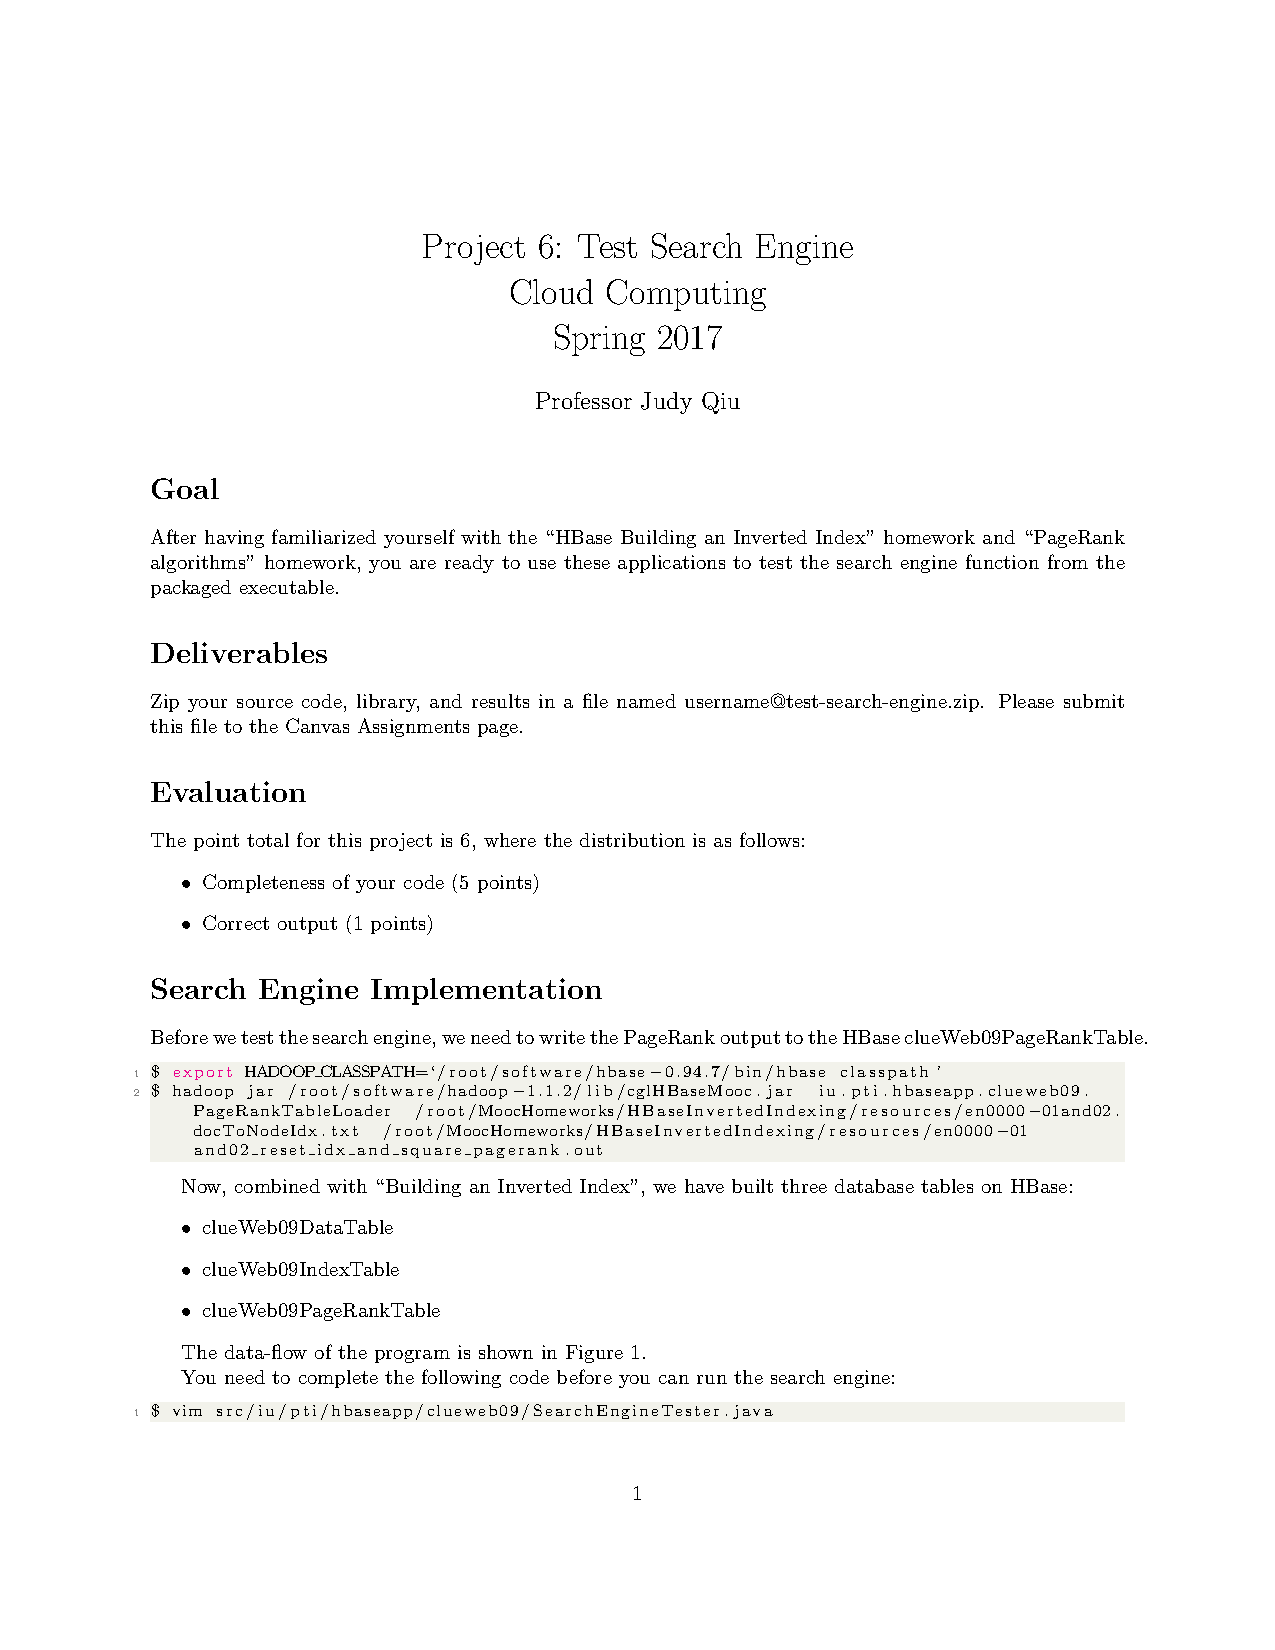
\includepdf[pages=-,pagecommand={},width=\textwidth]{section/icloud/assignment/files/project6.pdf}

\chapter{Project 7}\label{project-7}

The goal of this project is to familiarize yourself with the concept of
map-collective applications. Harp is similar to MapReduce in terms of
programming with the exception that it provides collective communication
support across map tasks.

Zip your source code and output as username\_harp-pagerank.zip. Please
submit this file to the Assignments page.

The point total for this project is 6, where the distribution is as
follows:

\begin{itemize}
\tightlist
\item
  Completeness of your code (5 points)
\item
  Correct output (1 point)
\end{itemize}

We prepared a new VM for project7 and project8. Please download it from
\href{https://drive.google.com/file/d/0B2iFsq4CY1DteHhJUEk5cDNJajQ/view}{here}.

\begin{itemize}
\tightlist
\item
  \href{https://drive.google.com/file/d/0B2iFsq4CY1DteHhJUEk5cDNJajQ/view}{VirtualBox
  VM Download}
\end{itemize}

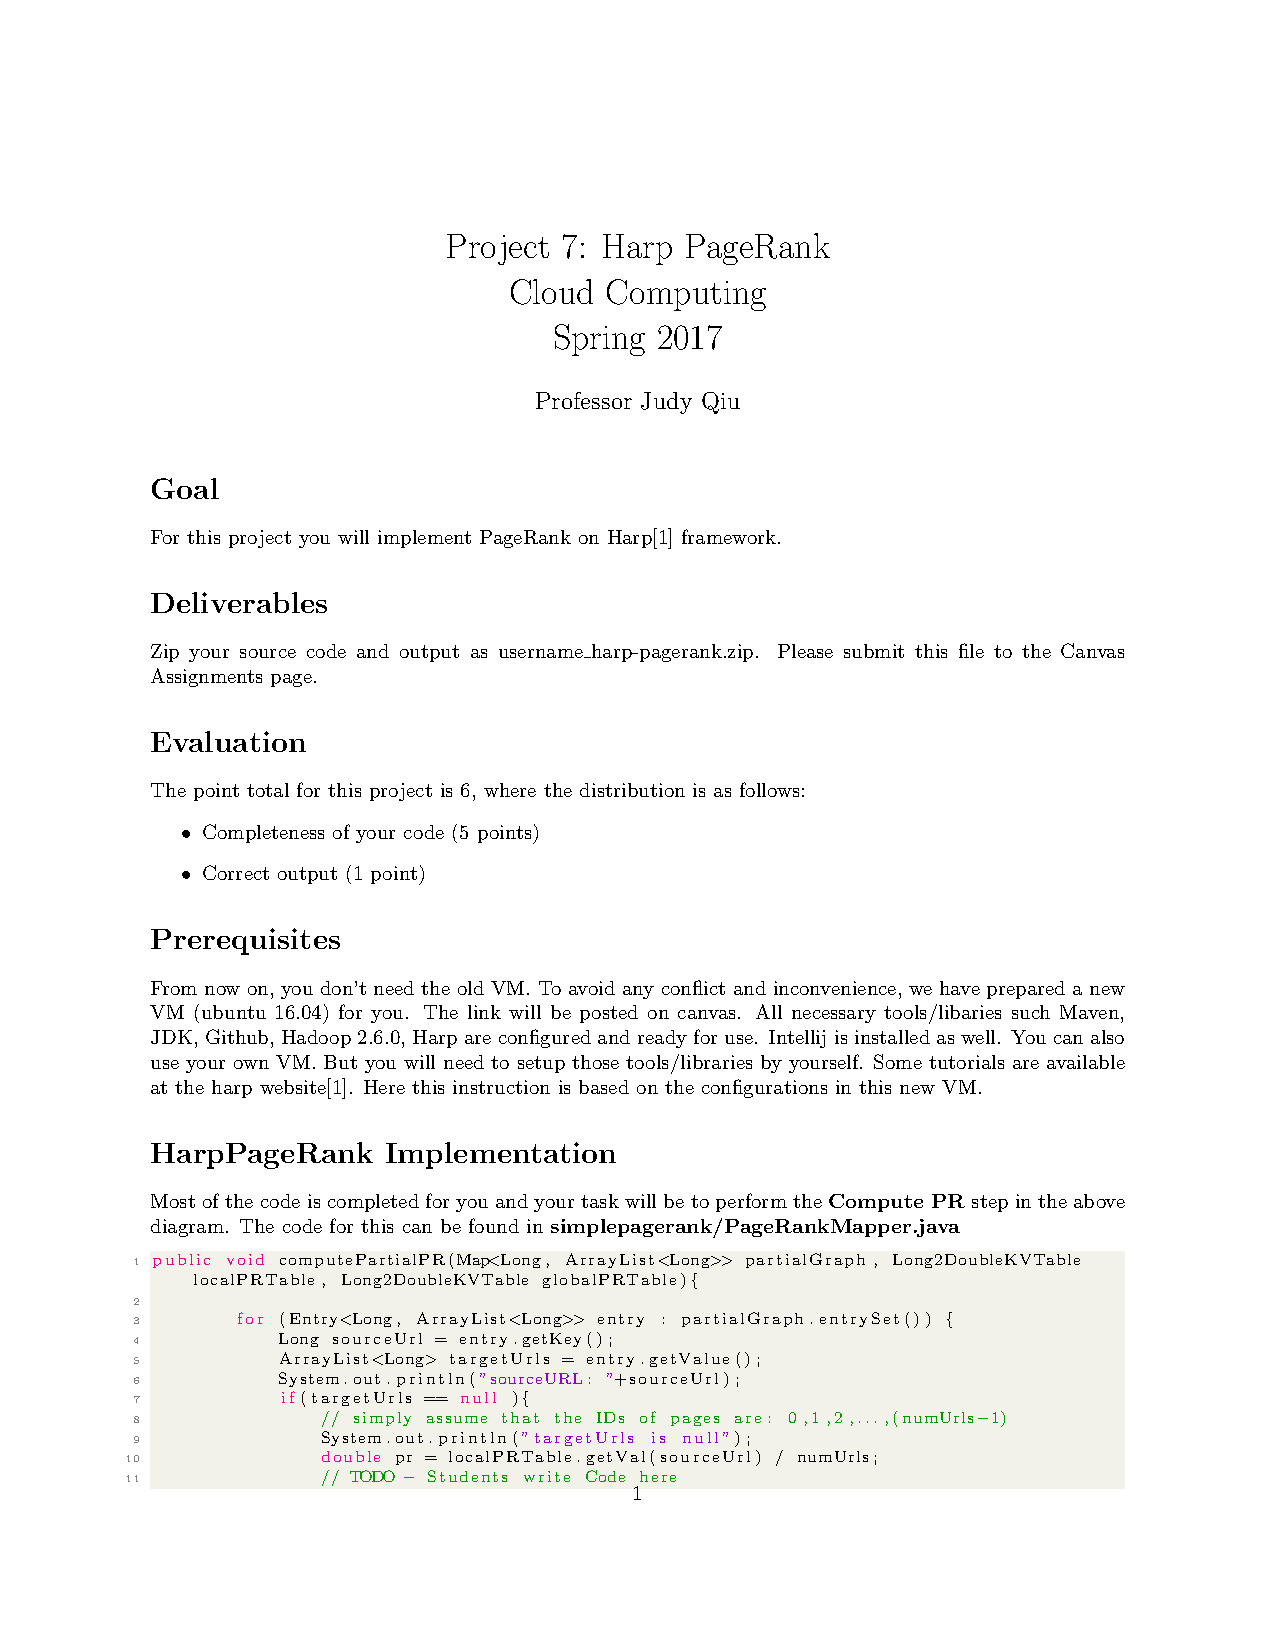
\includepdf[pages=-,pagecommand={},width=\textwidth]{section/icloud/assignment/files/project7.pdf}

\begin{description}
\item[Do not copy and paste commands from pdf files. Please type them]
manually. Special characters cause problems in executing commands in a
terminal.
\end{description}

\chapter{Project 8}\label{project-8}

Zip your source code and report as username\_mbkmeans.zip.

The point total for this project is 6, where the distribution is as
follows: - Completeness of your code (5 points) - In the report,
describe your implementation and the output. (1 points)

You can get up to 4 bonus points based on your extra efforts.

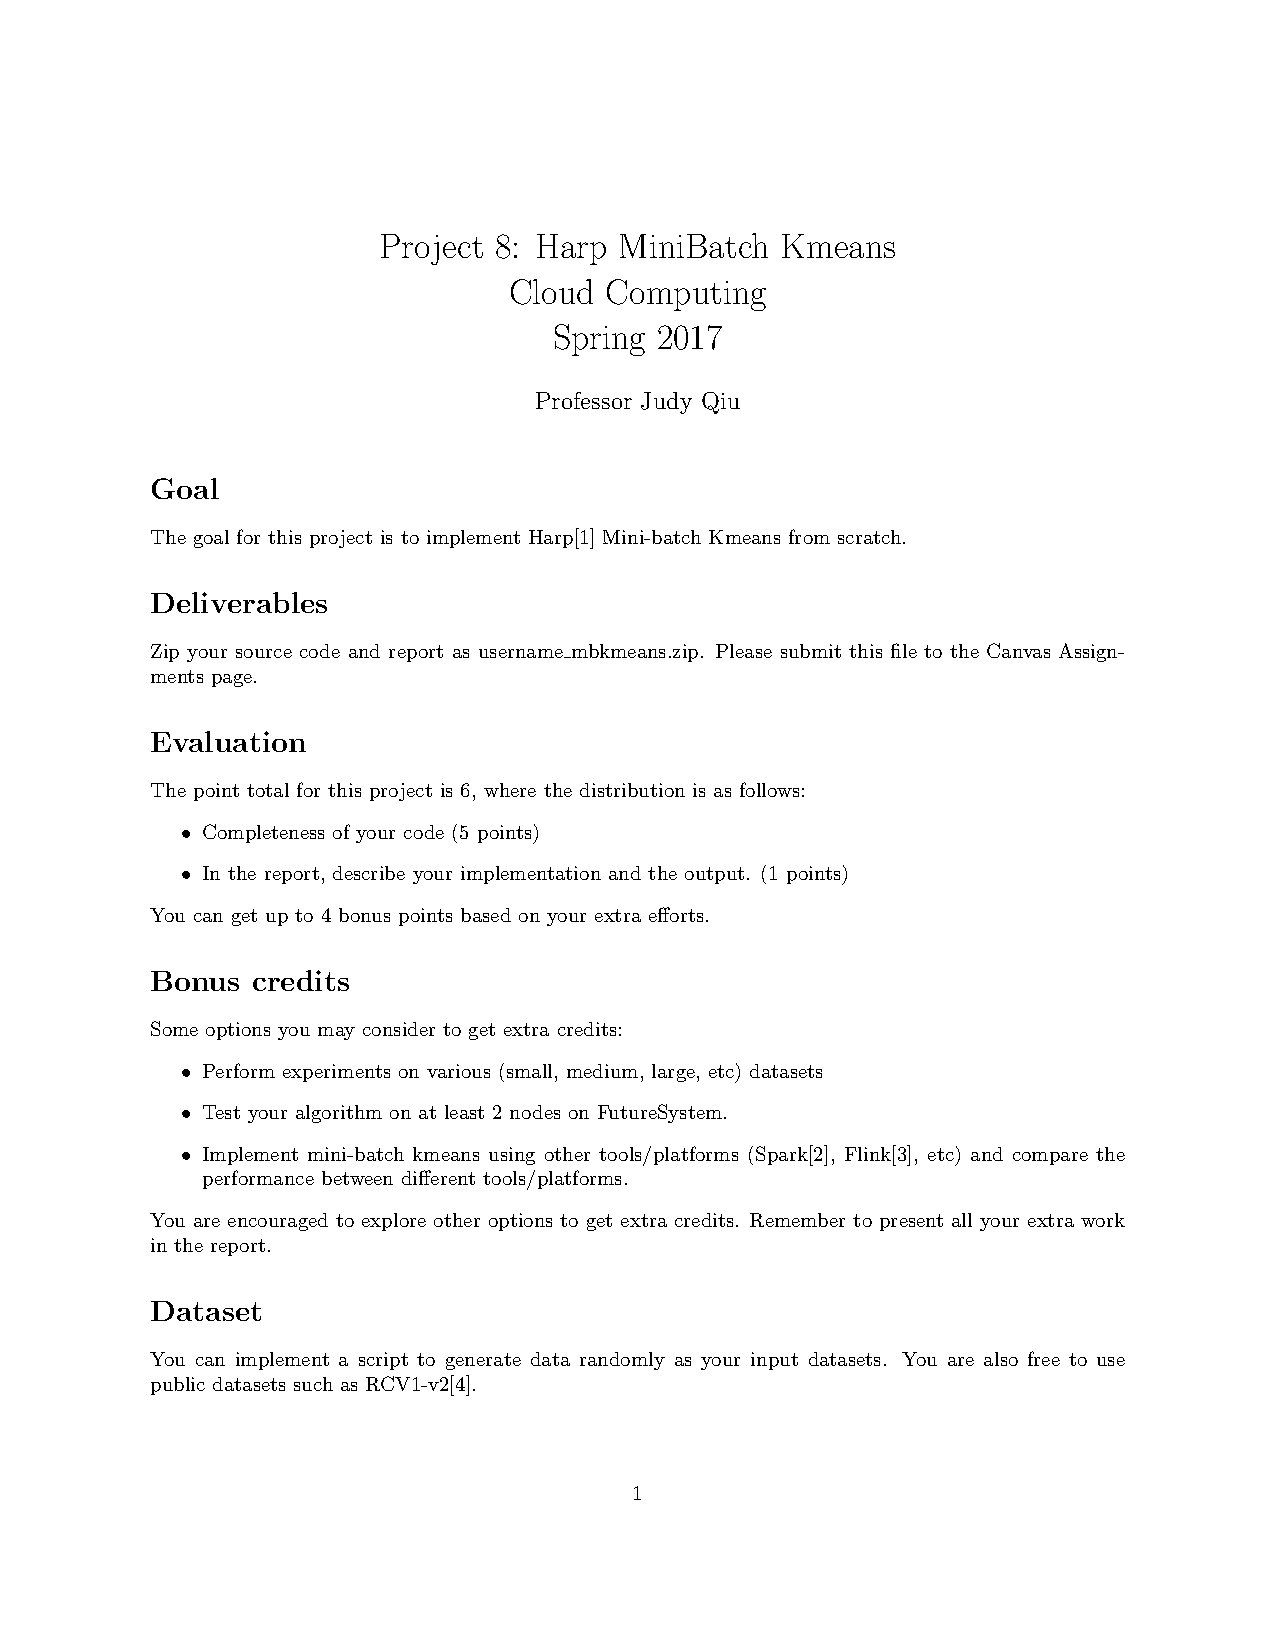
\includepdf[pages=-,pagecommand={},width=\textwidth]{section/icloud/assignment/files/project8.pdf}
